% (c) Egor Osipov

\documentclass[a4paper,12pt]{article} % тип документа (report, book)
\usepackage[14pt]{extsizes}
\usepackage[left=2cm,right=2cm, top=2cm,bottom=2cm,bindingoffset=0cm]{geometry} % Настройки документа
\usepackage{pgfplots}
\usepackage{pgfplotstable}
\usepackage{tikz} 

%  Русский язык
\usepackage[T2A]{fontenc}			% кодировка
\usepackage[utf8]{inputenc}			% кодировка исходного текста
\usepackage[english,russian]{babel}	% локализация и переносы


% Математика
\usepackage{amsmath,amsfonts,amssymb,amsthm,mathtools} 

% Просто смайлики
\usepackage{wasysym}

%Вставка картинок
\usepackage{graphicx}
\graphicspath{./}
\DeclareGraphicsExtensions{.pdf,.png,.jpg}
\usepackage{float}

% Настройка абзацев
\usepackage{indentfirst}
%\setlength{\parindent}{5ex}
%\setlength{\parskip}{1em}

\begin{document} % начало документа

%Заговолок
\begin{titlepage}
\begin{center}
	\large{Московский физико-технический институт}\\
	\vspace{100px}
	\LARGE{Работа 4.2.3}\\
	\LARGE{Интерферометр Релея.}\\
	\vspace{30px}
	
\includegraphics[scale = 0.3]{fakt_logo.png}\\
\end{center}

\vfill
\begin{flushright}
	\text{Осипов Егор. Б03-005}\\
	\text{г. Долгопрудный}
\end{flushright}
\end{titlepage}

\newpage

\tableofcontents

\newpage

\section{Цель работы и приборы.}

Ознакомление с устройством и принципом действия интерферометра Релея и с его применением для измерения показателя преломления газов.

\section{В работе используются.}

Технический интерферометр ИТР-1, светофильтр, баллог с углекислым газом, сильфон, манометр, краны.

В работе используется диффракция Фраунгофера на двух щелях.

\section{Теоритическая часть.}

\subsection{Введение.}

В интерферометре Релея используется дифракция Фраунгофера на двух щелях.
Используя принцип Гюйгенса-Френеля рассчитаем интенсивность световых колеба-
ний в волне, направление распространения которой составляет угол $\phi$ с нормалью к
экрану. Элемент щели dx посылает в направлении $\phi$ волну с амплитудой, пропорцио-
нальной dx. Фаза волны, приходящей в точку наблюдения от элемента с координатой
x, отстает от фазы волны, приходящей с $x = 0$, на величину $kx \sin(\phi)$. Колебание dE
в точка наблюдения, вызванное элементом dx, может быть записано в виде:

\begin{equation}
    dE = a \cos(\omega t - kx \sin \phi) dx
\end{equation}

Найдем результат 𝐸 суммарного действия всех элементов обоих щелей. Будем
при этом считать, что в правой щели создана дополнительная разность хода,
одинаковая для всех ее элементов. Интегрируя, получим:

\begin{equation}
    E = \int\limits_0^b a \cos(\omega t - kx \phi) dx +
    \int \limits_d^{d + b} a \cos(\omega t - kx\phi - k\vartriangle)dx
\end{equation}
Получаем:
\begin{center}
    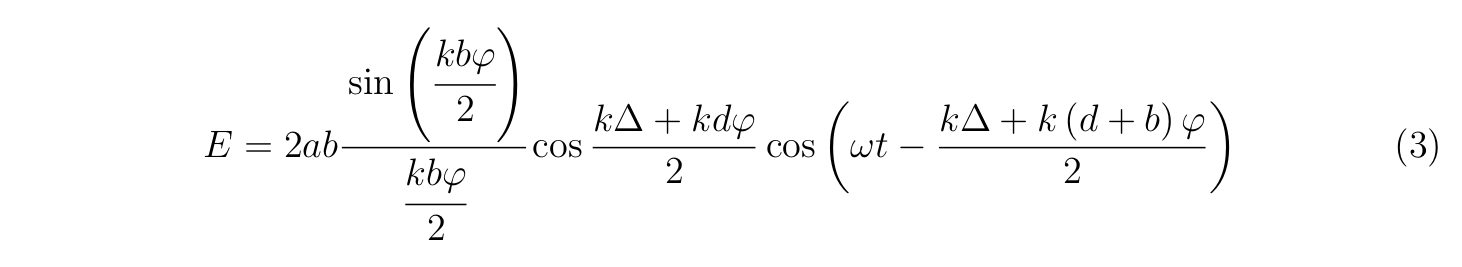
\includegraphics[scale = 0.4]{eq1}
\end{center}
Отсюда интенсивность:
\begin{center}
    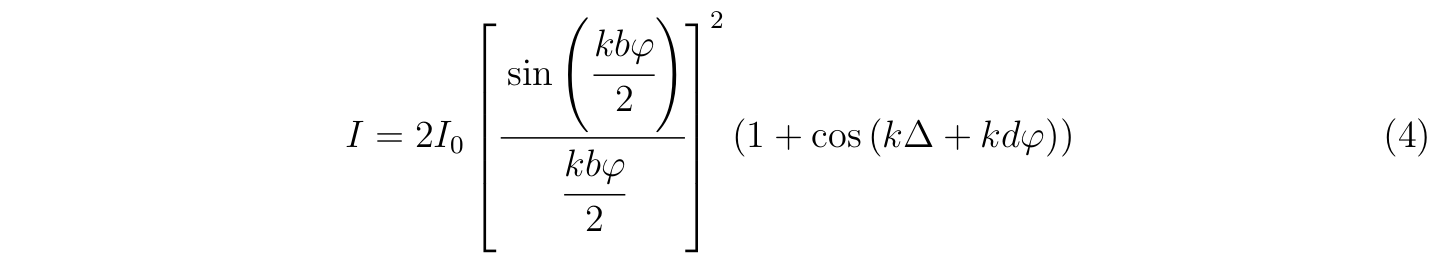
\includegraphics[scale = 0.4]{eq2}
\end{center}

Интерференционные максимумы отстоят друг от друга на равные угловые расстояния:

\begin{center}
    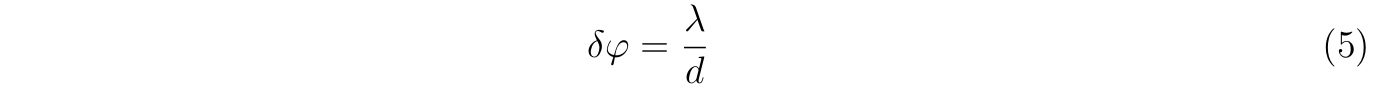
\includegraphics[scale = 0.4]{eq3}
\end{center}

\subsection{Описание установки.}

Схема прибора представлена на рисунке 1 в вертикальной и горизонтальной проекциях. Лампа накаливания Л с помощью конденсора К ярко освещает узкую входную щель S, расположенную в фокусе объектива $O_1$. Коллиматор, состоящий из
щели 𝑆 и объектива $O_1$, посылает параллельный пучок на диафрагму D с двумя
вертикальными щелями. Свет, дифрагируя на двойной щели проходит кювету L,
состоящую из двух одинаковых стеклянных камер, в которые вводятся исследуемые
газы. Кювета занимает только верхнюю часть пространства между объективами. За
кюветой расположены две стеклянных пластинки J и пластинка П.

Дифракционная картина, образующая в фокальной плоскости F объектива $O_2$,
рассматривается через окуляр $O$.

\begin{center}
    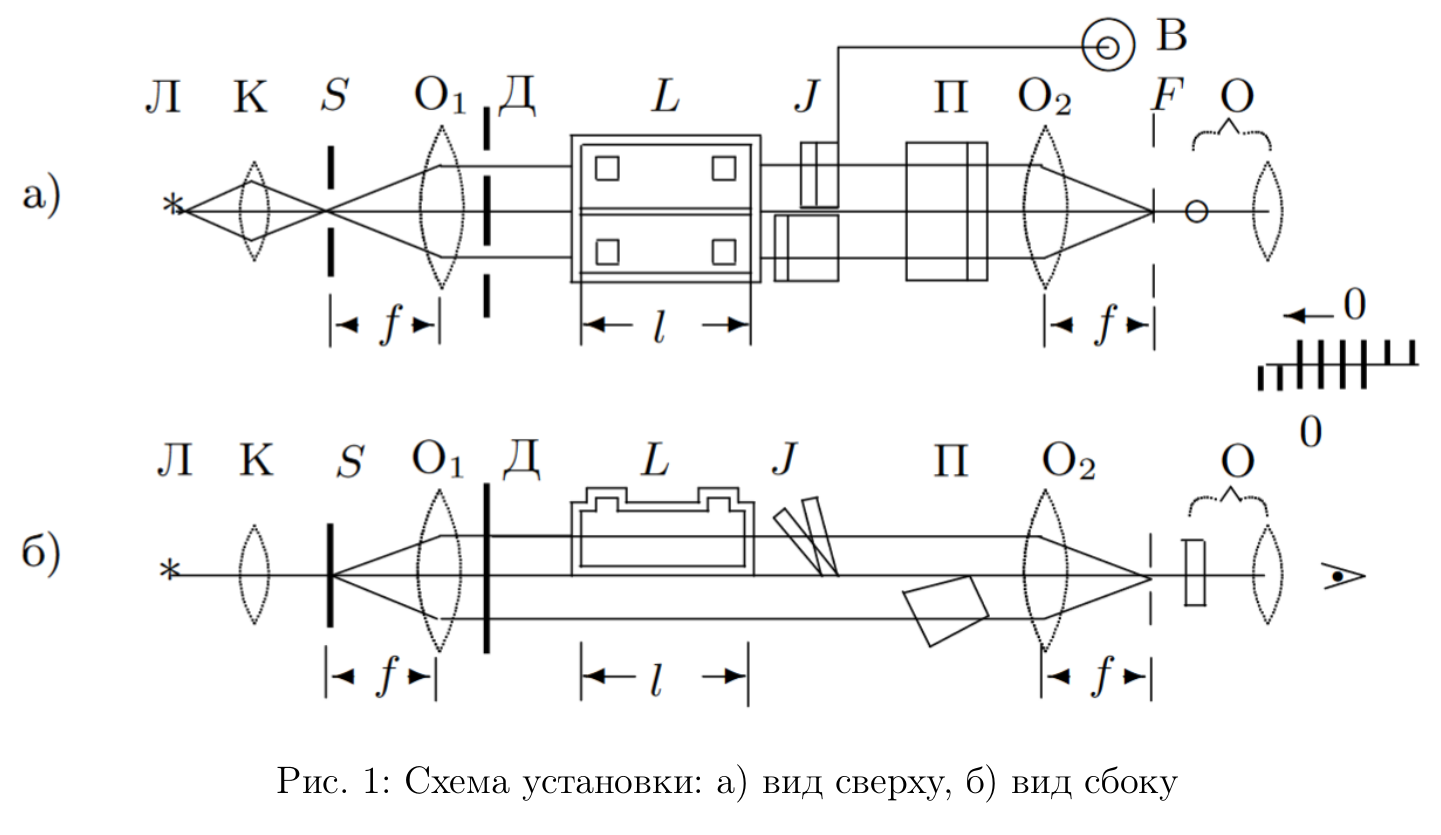
\includegraphics[scale=0.4]{pic1}
\end{center}

При заполнение камер газами с одинаковым показателем преломления 𝑛 системы
полос совпадают. Разность хода $\vartriangle = \vartriangle \text{n} * l$, возникает при прохождении света через
камеры с разными газами и ведет к смещению полос. Смещение на одну полосу
соответствует дополнительной разности хода $\vartriangle = \lambda$. Просчитав число полос между
центрами можно рассчитать:

\begin{center}
    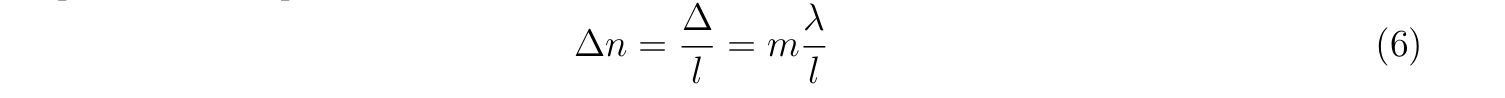
\includegraphics[scale=0.4]{eq4}
\end{center}

\subsection{Зависимость показателя преломления газа от давления и температуры.}

Известно простое соотношение между показателем преломления газа и его плот-
ностью:

\begin{center}
    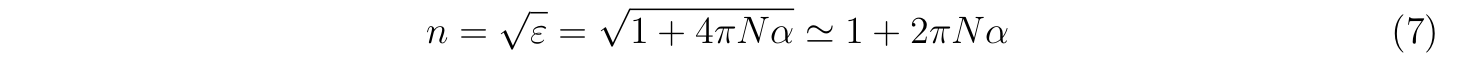
\includegraphics[scale=0.4]{eq5}
\end{center}
Принимая во внимание $p = NkT$, получим:

\begin{center}
    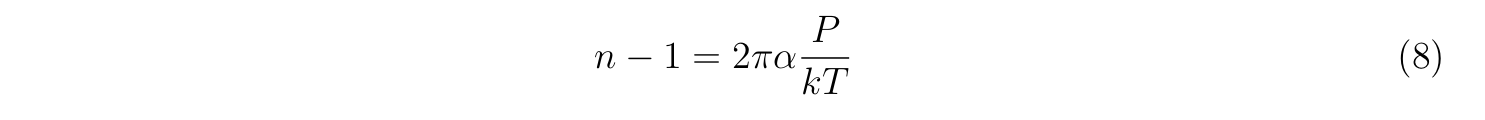
\includegraphics[scale=0.4]{eq6}
\end{center}

Отсюда следует, что при постоянной температуре изменение показателя преломле-
ния $\vartriangle$n пропорционально изменению давления $\vartriangle$P.

\begin{center}
    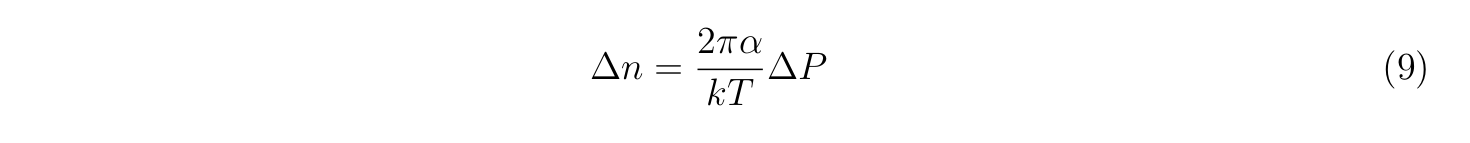
\includegraphics[scale=0.4]{eq7}
\end{center}

\section{Экспериментальная часть.}

Длина кюветы l = 10 см, атмосферное давление $P = 101.2 \cdot 10^3$Па, температу-
ра $T = 21^\circ C$. Прокалибруем установку в единицах $lambda$. Для этого построим график
смещения от номера полосы:
 
\begin{center}
    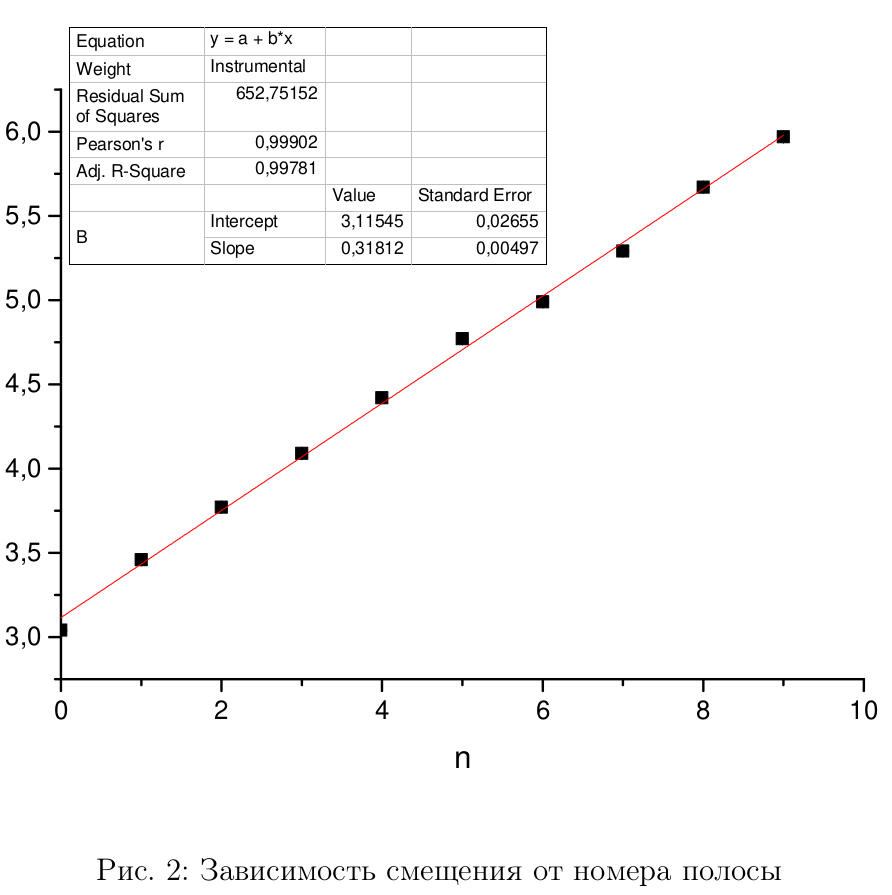
\includegraphics[scale=0.6]{pic2}
\end{center}

Будем использовать калибровочный график для расчета $\vartriangle$n. Таким образом построим график $\vartriangle$n($\vartriangle$P)

\begin{center}
    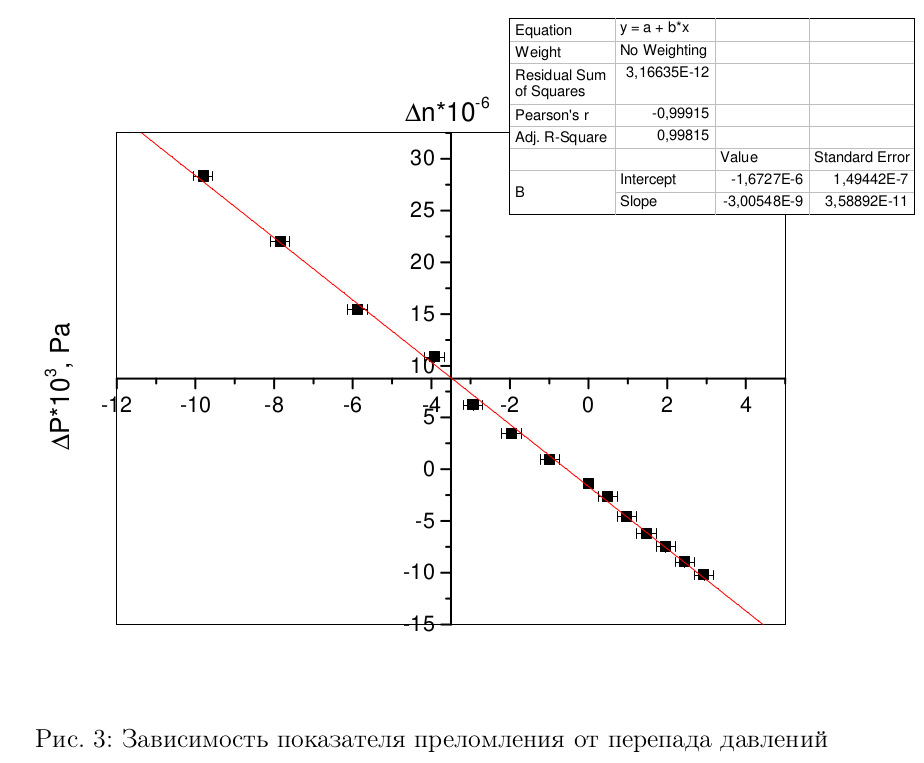
\includegraphics[scale=0.7]{pic3}
\end{center}

Отсюда получаем показатель преломления воздуха. пересчитанный к нормаль-
ным условиям $n_0 = 1.0003 \pm 0.00005$, что сходится с табличным результатом в 
пределах погрешности ($n_0t = 1.0002929$).

Теперь заполним кювету углекислым газом, и пронаблюдаем зависимость сме-
щения компенсатора от времени:

Равновесие устанавливается очень долго, следовательно концентрация $CO_2$ в
каждый момент времени не очень понятна. Поэтому будем заполнять кювету уг-
лекислым газом медленно, во избежание изменения температуры при расширении
газа и рассчитаем показатель преломления по одной начальной точке:

\begin{center}
    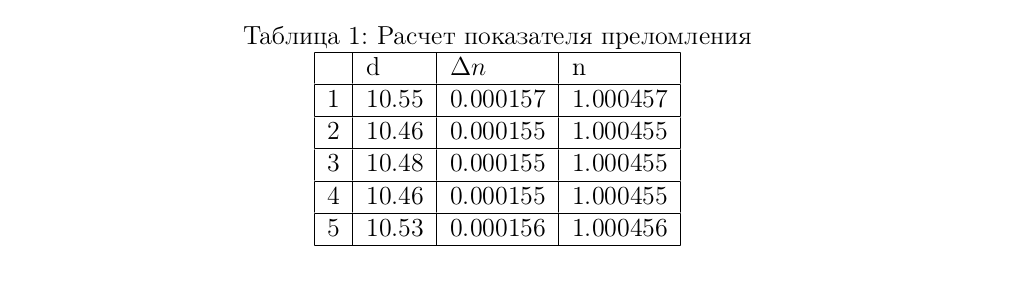
\includegraphics[scale=0.6]{tab1}
\end{center}

\begin{center}
    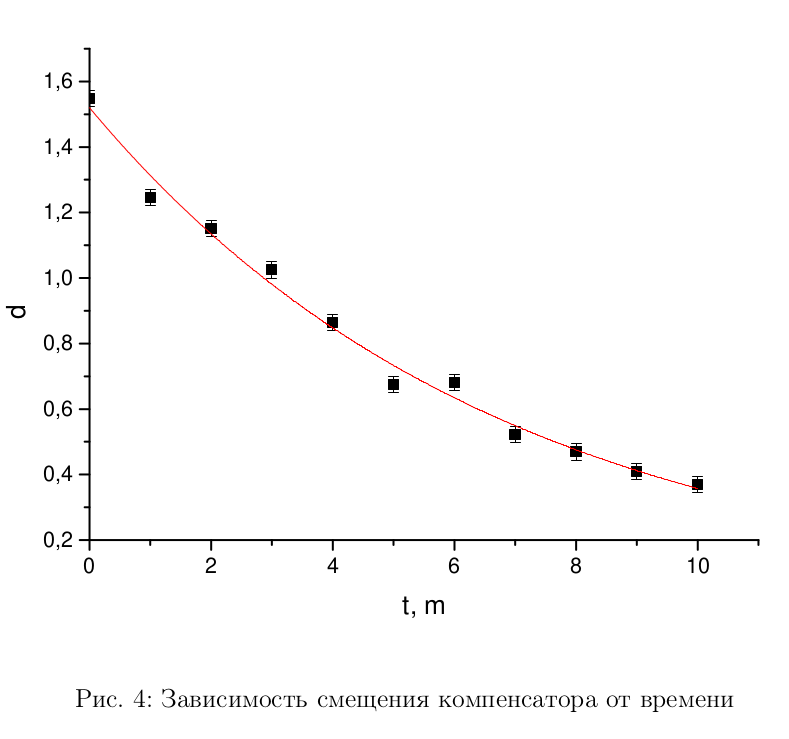
\includegraphics[scale=0.8]{pic4}
\end{center}

Итого $n = 1.00045 \pm 0.00002$. Табличный показатель преломления для $CO_2$: $n_0 = 1.00045$, что также сходится с нашими измерениями.

\section{Вывод.}

Интерферометр Релея позволяет измерять разность показателей преломления
в двух кюветах с высокой точностью. Для таких измерений нужно поддерживать
давление в кюветах и концентрацию газа постоянной, в противном случае точность
и простота измерений значительно ухудшаются.

\end{document} % конец документа
